\section{Tervezés és architektúra}

\indent Az alkalmazás fejlesztése során célkitűzésem az volt, hogy egy jól strukturált, skálázható és hosszú távon is fenntartható rendszert hozzak létre, amely modern fejlesztési elvekre épül. A rendszer célja, hogy egyszerűsítse a buszjáratok kezelését, a menetrendek nyilvántartását, valamint megkönnyítse a jegyvásárlás és adminisztratív tevékenységek lebonyolítását. Ebben a fejezetben bemutatom a rendszer architektúráját, az adatbázis-tervet, az entitások kapcsolatrendszerét, valamint a tervezés során hozott döntéseket.

\subsection{Rendszerarchitektúra}

\indent Az alkalmazás háromrétegű architektúrát követ, amely a prezentációs, alkalmazáslogikai és adatelérési rétegeket világosan elkülöníti. Ez a struktúra lehetővé teszi a moduláris fejlesztést, a különböző rétegek független tesztelhetőségét, valamint az egyszerű jövőbeli módosításokat és bővítéseket.

\begin{itemize}
    \item \textbf{Prezentációs réteg (View)} – A felhasználói felület ASP.NET MVC technológiával készült, Razor nézetek alkalmazásával. A cél egy átlátható, reszponzív és intuitív felhasználói élmény biztosítása volt. Az oldal struktúrája a Bootstrap keretrendszerre épül, ezzel támogatva a mobileszközökön való megjelenést is.
    
    \item \textbf{Alkalmazáslogikai réteg (Controller + Business Logic)} – Ez a réteg felel az üzleti szabályok érvényesítéséért, az adatok feldolgozásáért és a logikai műveletekért. A kontroller osztályok kommunikálnak az adatelérési réteggel, és ellátják az adatokat a nézetek számára. A rendszer szerepköralapú hitelesítést használ az ASP.NET Identity segítségével.

    \item \textbf{Adatelérési réteg (Data Access Layer)} – Az adatok tárolása SQL Server-ben történik, míg a kommunikáció az Entity Framework Core ORM-en keresztül valósul meg. Ez lehetővé teszi az objektum-orientált adatkezelést, a LINQ-alapú lekérdezéseket és az adatbázis sémájának migrációját.
\end{itemize}

\subsection{Adatbázis-tervezés}

\indent A rendszer adatbázisa relációs sémára épül, amely biztosítja a konzisztens adatkezelést és a gyors lekérdezéseket. A táblák között többféle kapcsolat (egy-a-többhöz, több-a-többhöz) került kialakításra, figyelembe véve a normalizálási szabályokat.
\newpage
\subsubsection{Adatmodell – entitások bemutatása}

Az alábbiakban bemutatom az alkalmazásban használt főbb entitásokat, azok mezőit, adattípusait és a mezők rendeltetését.

\paragraph{Contact}

A \texttt{Contact} entitás a rendszer regisztrált felhasználóit reprezentálja, és az ASP.NET Identity rendszer \texttt{IdentityUser} osztályából származik. Ezáltal örökli annak számos beépített mezőjét és funkcionalitását, mint például a felhasználónév (\texttt{UserName}), e-mail cím (\texttt{Email}), jelszó hash (\texttt{PasswordHash}), valamint a fiók zárolással, biztonsági tokenekkel, e-mail és telefonszám megerősítéssel kapcsolatos mezőket.

\paragraph{Contact}

A rendszer felhasználóit reprezentáló alapvető entitás a \texttt{Contact} osztály, amely az ASP.NET Identity infrastruktúrájára épül, pontosabban az \texttt{IdentityUser} osztályból származik. Ez az öröklődés lehetővé teszi a beépített azonosítási és hitelesítési funkciók használatát, például a felhasználónév, az e-mail cím, a jelszótárolás hash formátumban, valamint a különféle biztonsági funkciók – mint például fiókzárolás, e-mail- és telefonszám-ellenőrzés – elérését.

A projekt specifikus igényeihez igazodva a \texttt{Contact} entitás további mezőkkel került kibővítésre. Minden felhasználó egy egyedi azonosítóval rendelkezik, amely GUID formátumban kerül tárolásra, ez biztosítja az entitás egyértelmű beazonosíthatóságát. A felhasználók teljes neve külön mezőben kap helyet, amely az azonosításon túl a különböző nézetekben és riportokban való megjelenítést is szolgálja. A rendszer az e-mail címet elsődleges kapcsolattartási pontként használja, emellett lehetőség van telefonszám megadására is, amely főként közvetlen kommunikáció esetén hasznos. Az egyes felhasználók szerepköre – legyen az például adminisztrátor, munkatárs vagy ügyfél – szöveges formában kerül rögzítésre, ez határozza meg, hogy milyen jogosultságokkal rendelkeznek a rendszerben. A jelszavak biztonságos tárolását a keretrendszer által biztosított hash-elési mechanizmus kezeli.

A hozzáférések szabályozása szerepkör-alapú logikát követ, így minden felhasználó csak az általa betöltött szerephez tartozó funkciókat érheti el. Bár az ASP.NET Identity rendszer lehetőséget kínál összetettebb jogosultságmodellek kialakítására az \texttt{IdentityRole} és \texttt{UserRole} entitásokon keresztül, a jelen fejlesztés során egy egyszerűsített megoldás került alkalmazásra, amelyben a szerepkörök egyetlen szöveges mezőben kerülnek tárolásra.

A regisztráció, bejelentkezés, jelszómódosítás, illetve a biztonsággal kapcsolatos funkciók – mint például az e-mail visszaigazolás vagy a többszöri sikertelen belépési kísérlet utáni fiókzárolás – mind az ASP.NET Identity keretrendszer alapvető elemeire épülnek. Ezáltal biztosított a felhasználói adatok megbízható kezelése és a rendszerbe való belépések megfelelő védelme.


\paragraph{Bus}

A \texttt{Bus} entitás az egyes autóbuszokat írja le. A \texttt{BusId} (\textit{string}) az egyedi azonosító, míg a \texttt{LicensePlate} mező (\textit{string}) a busz rendszámát tartalmazza. A \texttt{Capacity} mező (\textit{int}) az ülőhelyek számát rögzíti, a \texttt{BusType} mező (\textit{string}) pedig a jármű típusát jelzi, például városi vagy távolsági busz.

\paragraph{Stop}

A \texttt{Stop} entitás egy-egy megállóhelyet reprezentál. Az \texttt{StopId} mező (\textit{string}) az adott megálló egyedi azonosítója. A \texttt{Name} mező (\textit{string}) a megálló nevét, míg a \texttt{Latitude} és \texttt{Longitude} mezők (\textit{double}) a földrajzi koordinátákat – szélességi és hosszúsági adatokat – tárolják.

\paragraph{TransportRoute}

A \texttt{TransportRoute} entitás egy közlekedési útvonalat reprezentál. A \texttt{TransportRouteId} mező (\textit{string}) az útvonal egyedi azonosítója, a \texttt{Name} mező (\textit{string}) pedig az útvonal nevét tartalmazza. A \texttt{StartStopId} és \texttt{EndStopId} mezők (\textit{string}) az induló és végállomások azonosítóit rögzítik.

\paragraph{RouteStop}

A \texttt{RouteStop} entitás egy kapcsolatot képez a megállók és az útvonalak között, ezzel lehetővé téve az egyes útvonalakhoz tartozó megállók sorrendjének meghatározását. Az \texttt{RouteStopId} (\textit{string}) azonosítja az entitást, a \texttt{TransportRouteId} (\textit{string}) a kapcsolódó útvonalra, míg a \texttt{StopId} (\textit{string}) az adott megállóra mutat. Az \texttt{Order} mező (\textit{int}) az adott megálló sorszámát jelzi az útvonalon belül.

\paragraph{Schedule}

A \texttt{Schedule} entitás a menetrendi adatokat tárolja. Az \texttt{ScheduleId} mező (\textit{string}) az egyedi azonosító, a \texttt{TransportRouteId} (\textit{string}) és \texttt{BusId} (\textit{string}) mezők a kapcsolódó útvonalat és autóbuszt azonosítják. A \texttt{DepartureTime} mező (\textit{DateTime}) az indulás pontos időpontját rögzíti.

\paragraph{Ticket}

A \texttt{Ticket} entitás az utasok által megvásárolt jegyeket reprezentálja. A \texttt{TicketId} mező (\textit{string}) az egyedi azonosító, a \texttt{ScheduleId} (\textit{string}) a kapcsolódó menetrendre, a \texttt{PassengerId} (\textit{string}) pedig a jegyet vásárló utasra (Contact) hivatkozik. A \texttt{SeatNumber} mező (\textit{int}) az adott jegyhez tartozó ülőhely számát, míg a \texttt{PurchaseDate} (\textit{DateTime}) a vásárlás időpontját tartalmazza.

\paragraph{AdminMessage}

Az \texttt{AdminMessage} entitás a látogatók vagy felhasználók által küldött üzeneteket tárolja. Az \texttt{AdminMessageId} mező (\textit{string}) az egyedi azonosító, a \texttt{Name} és \texttt{Email} mezők (\textit{string}) az üzenet küldőjének nevét és e-mail címét tartalmazzák. A \texttt{Message} mező (\textit{string}) az üzenet szövegét, a \texttt{SentAt} mező (\textit{DateTime}) pedig annak elküldési időpontját rögzíti.

\paragraph{AdminTask}

Az \texttt{AdminTask} entitás az adminisztrátori feladatokat tárolja. Az \texttt{AdminTaskId} mező (\textit{string}) az egyedi azonosító, a \texttt{Title} és \texttt{Description} mezők (\textit{string}) a feladat nevét és részletes leírását tartalmazzák. A \texttt{CreatedAt} mező (\textit{DateTime}) a létrehozás időpontját, míg az \texttt{AssignedToId} mező (\textit{string}) a felelős adminisztrátorra (Contact) történő hivatkozást tartalmazza.

\paragraph{Attachment}

Az \texttt{Attachment} entitás fájlmellékleteket ír le. Az \texttt{AttachmentId} mező (\textit{string}) egyedi azonosítóként szolgál, a \texttt{FileName} (\textit{string}) a feltöltött fájl nevét, a \texttt{FilePath} (\textit{string}) pedig annak szerveren való elérési útját tartalmazza. A \texttt{UploadedAt} mező (\textit{DateTime}) a feltöltés időpontját, míg az \texttt{UploadedById} mező (\textit{string}) a feltöltést végző felhasználóra (Contact) való hivatkozást jelenti.


\subsubsection{Táblakapcsolatok}

A rendszer relációs adatmodellje több különböző típusú kapcsolatot valósít meg az entitások között, figyelembe véve az alkalmazás logikai működését és az adatintegritás követelményeit. A modellben több egy-a-többhöz (1:N) kapcsolat is megtalálható. Például egy regisztrált felhasználó – akit a \texttt{Contact} entitás reprezentál – több jegyet is birtokolhat, tehát a \texttt{Contact} és a \texttt{Ticket} entitások között 1:N típusú viszony áll fenn. Hasonló reláció létezik a \texttt{Bus} és a \texttt{Schedule} entitások között is, mivel egy adott jármű több menetrend szerint is közlekedhet.

Az útvonalakat alkotó megállók sorrendiségét a \texttt{RouteStop} entitás írja le, amely egy-egy megállót és egy-egy útvonalat köt össze. Ez az entitás két darab N:1 kapcsolatot is tartalmaz: minden \texttt{RouteStop} bejegyzés pontosan egy \texttt{Stop} és egy \texttt{TransportRoute} rekordhoz tartozik. Ezzel a struktúrával biztosítható az útvonalak szakaszainak pontos leképezése és a megállók sorrendjének rögzítése.

A \texttt{Schedule} entitás kettős hivatkozással kapcsolódik a \texttt{Bus} és a \texttt{TransportRoute} entitásokhoz. Minden menetrendi bejegyzéshez pontosan egy busz és egy útvonal tartozik, így ezen kapcsolatok mindegyike egy-egy 1:1 vagy 1:N viszonyt jelent, attól függően, hogy az adott jármű vagy útvonal hány különböző időpontban kerül beütemezésre.

\subsection{Entitások részletes modellezése}

Az alkalmazás modelljei világosan elkülönítik az egyes üzleti szereplőket és folyamatokat, az elvárt funkcionalitásnak megfelelő struktúrában. A \texttt{Ticket} entitás minden egyes példánya konkrét kapcsolatban áll egy felhasználóval (\texttt{Contact}) és egy menetrendi bejegyzéssel (\texttt{Schedule}), valamint egy rendszer által generált ülőhelyszámmal. Ez biztosítja a tranzakciók egyértelmű követhetőségét.

Az útvonalakat részletező \texttt{RouteStop} entitás lehetőséget nyújt a megállók sorrendi rendezésére az adott útvonalon belül, amely különösen hasznos a vizuális megjelenítés vagy térképes lekövetés során. A dokumentumok kezelése céljából létrehozott \texttt{Attachment} entitás lehetőséget ad fájlok feltöltésére és rendszerezésére, például adminisztratív vagy ügyfélszolgálati célból. A \texttt{AdminMessage} és \texttt{AdminTask} entitások a háttérrendszert támogató funkciók megvalósítását szolgálják: előbbi az üzemeltetői kommunikációt, utóbbi a feladatok kijelölését és nyomon követését teszi lehetővé.

\subsection{Adatbázis entitásdiagram}

\begin{figure}[H]
    \centering
    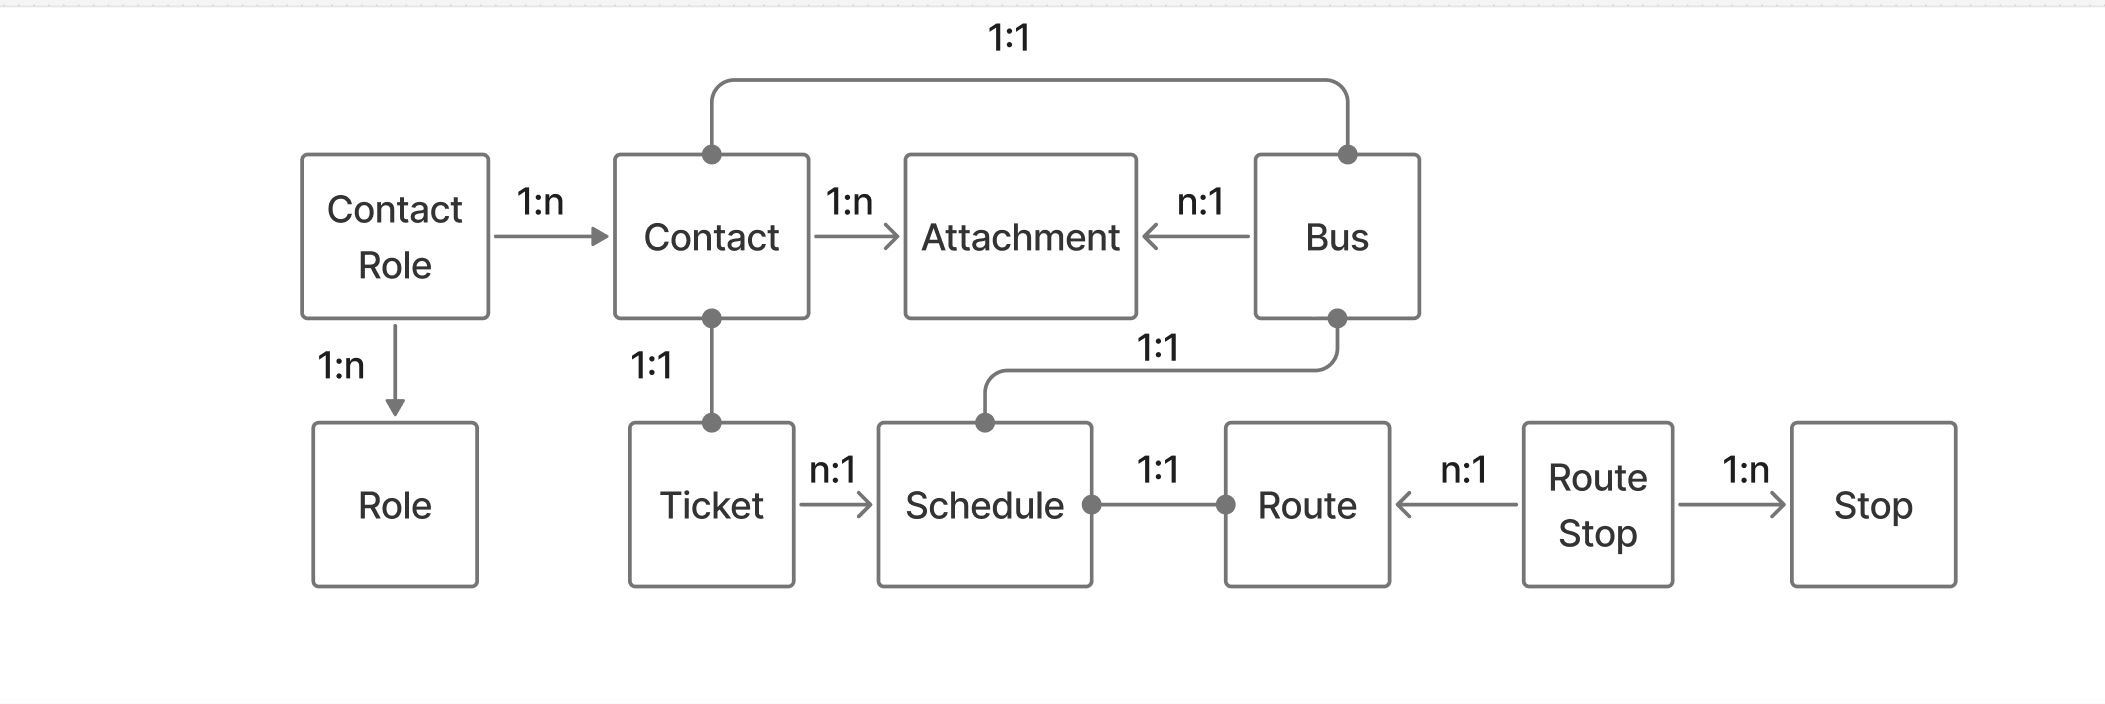
\includegraphics[width=1\textwidth]{Szakdolgozat/Mellekletek/ERdiagram.PNG}
    

    \caption{Az adatbázis entitás-kapcsolat (E-K) diagramja}
    \label{fig:er-diagram}
\end{figure}

A \ref{fig:er-diagram}. ábrán látható az adatbázis logikai struktúrája.


\subsection{Felhasználói felület}

\indent A webalkalmazás felhasználói felületének kialakítása során elsődleges szempont volt az átláthatóság, a reszponzivitás, valamint a felhasználóbarát működés. A rendszer minden látogató számára egységes struktúrát biztosít, azonban a megjelenített tartalom és a hozzáférhető funkciók dinamikusan változnak a bejelentkezési állapot és a felhasználói szerepkör függvényében. A felület úgy került kialakításra, hogy mind a regisztrált utasok, mind az adminisztrátori jogosultsággal rendelkező felhasználók számára a szerepkörükkel releváns tartalom jelenjen meg.

\subsubsection{Főoldal}

\indent A kezdőlap minden látogató számára elérhető, és egy jól strukturált navigációs sávval segíti az alkalmazás fő funkcióinak gyors elérését. A menüsorban az alábbi pontok találhatók meg: \texttt{Stations}, \texttt{Routes}, \texttt{Schedules}, \texttt{MyTickets}, valamint a \texttt{Contact Us}. A jobb felső sarokban megjelenő opciók a látogató aktuális státuszától függenek. Be nem jelentkezett állapotban a \texttt{Login} és \texttt{Register} lehetőségek állnak rendelkezésre, míg bejelentkezett felhasználók esetében a \texttt{Profile} és a \texttt{Logout} gombok válnak láthatóvá. Amennyiben a bejelentkezett felhasználó adminisztrátori jogosultságokkal rendelkezik, egy további \texttt{Adminisztráció} legördülő menü is elérhetővé válik, amely az adminisztrációs funkciókhoz biztosít közvetlen hozzáférést.

\paragraph{Felhasználói nézet (utas szerepkör)}

\indent A rendszer általános felhasználói, azaz az utasok számára kialakított nézet célja, hogy a közlekedési szolgáltatások gyorsan és intuitív módon elérhetők legyenek. A kezdőoldalon keresztül megtekinthetők a vállalat által karbantartott megállók, amelyek földrajzi és logikai elhelyezkedésük alapján rendszerezettek. Az útvonalak menüpont segítségével a felhasználók megismerhetik az elérhető közlekedési útvonalakat, valamint az egyes útvonalakon szereplő megállókat is.

\indent A menetrendek áttekintése szintén kiemelt szerepet kap: az indulási időpontok, a járatokhoz tartozó útvonalak és a járművek együttesen jelennek meg, támogatva a tervezhető és hatékony utazást. A felhasználók számára elérhető a jegyvásárlási lehetőség is, amelyet vizuálisan kiemelt gomb segít megtalálni. A már megvásárolt jegyek a \texttt{MyTickets} szekcióban kerülnek listázásra, ahol a felhasználó saját jegyeit tekintheti át, függetlenül attól, hogy azok aktív vagy már lejárt foglalások. Ezen kívül a \texttt{Contact Us} menüpont egy kapcsolatfelvételi űrlapot biztosít, amelyen keresztül az adminisztráció számára üzenet küldhető, például észrevételek vagy kérdések esetén.

\indent Az egyszerű navigációs élmény részeként a jobb felső sarokban található profilmenü lehetőséget ad a személyes adatok megtekintésére és szerkesztésére. Ezáltal a felhasználók bármikor módosíthatják profiladataikat, illetve kijelentkezhetnek a rendszerből.

\paragraph{Adminisztrátori nézet}

\indent Az adminisztrátorok számára elérhető nézet jelentősen kibővített funkcionalitással rendelkezik. A bejelentkezést követően egy speciális \texttt{Adminisztráció} nevű legördülő menüpont válik aktívvá, amely az alkalmazás háttérrendszeréhez biztosít hozzáférést. Ennek segítségével az adminisztrátorok jogosultak új buszmegállók létrehozására, a meglévő megállók módosítására vagy törlésére. Az útvonalak karbantartása során lehetőség van új útvonalak definiálására, illetve a meglévők struktúrájának frissítésére.

\indent A menetrendek kezelése is része az adminisztrációs felületnek: az indulási időpontokhoz kapcsolódó adatok, valamint a jármű-hozzárendelések módosíthatók. A járműpark menedzselése során az autóbuszok nyilvántartása, adatszerkesztése és bővítése valósítható meg. Az adminisztrátorok hozzáférnek minden felhasználói jegyhez, így átfogó képet kapnak az utazási forgalomról.

\indent A rendszer lehetőséget biztosít a regisztrált felhasználók adatainak kezelésére is, beleértve az egyéni kapcsolattartási információkat és szerepköröket. A \texttt{ToDoList} funkció segítségével az adminisztrátorok belső feladatokat követhetnek nyomon. A beérkező felhasználói üzenetek külön felületen keresztül érhetők el, ahol válaszadásra is van lehetőség.

\indent További fontos adminisztratív funkció a szerepkörök kezelése: az adminisztrátorok új szerepköröket definiálhatnak, illetve módosíthatják a meglévőeket (pl. utas, alkalmazott, adminisztrátor), ezzel szabályozva a hozzáférési jogosultságokat az alkalmazás különböző moduljaihoz.

\indent Míg az utas szerepkörrel rendelkező felhasználók jellemzően csak megtekintési jogosultsággal rendelkeznek, addig az adminisztrátorok számára minden entitáson elérhetővé válik a teljes CRUD-funkcionalitás (Create, Read, Update, Delete). Ez a szerepköralapú jogosultságkezelés biztosítja, hogy a rendszer minden felhasználó számára csak az általa engedélyezett műveletek legyenek elérhetők, miközben a felület egységes marad.
\begin{figure}[H]
    \centering
    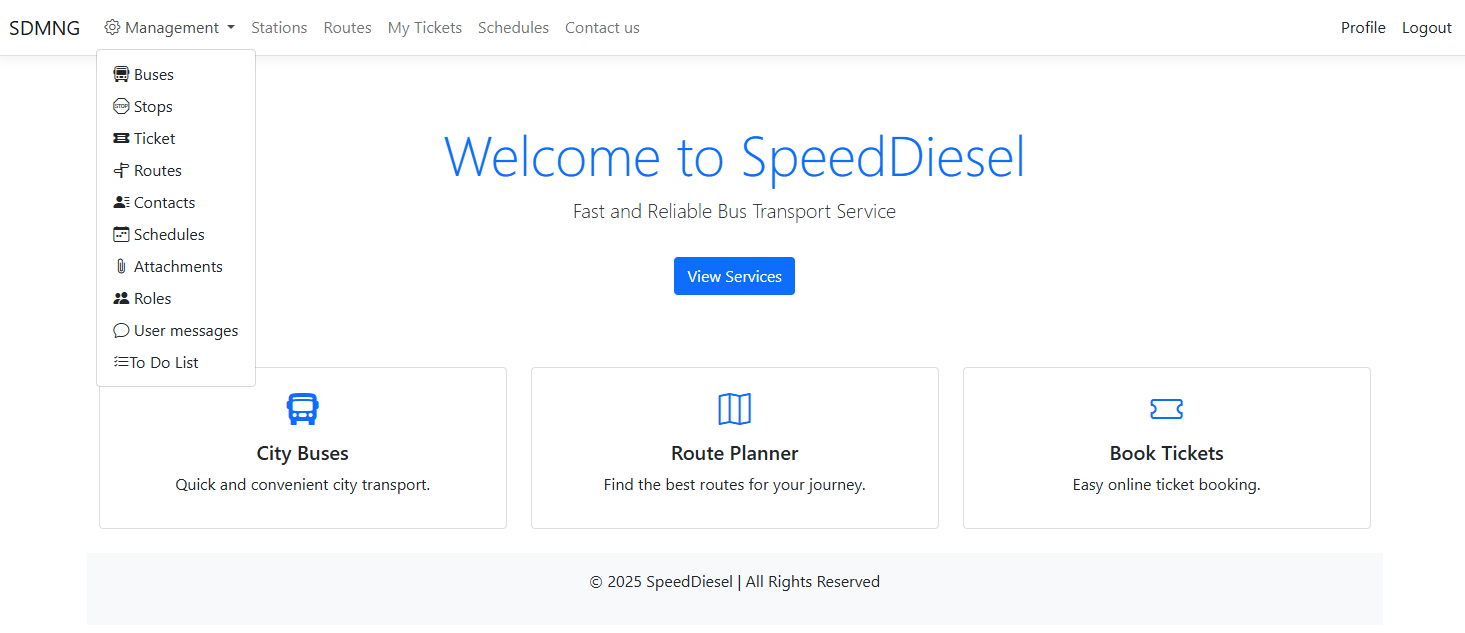
\includegraphics[width=1\textwidth]{Szakdolgozat/Mellekletek/fooldal.PNG}
    \caption{A rendszer főoldala adminisztrátori bejelentkezés után, látható \texttt{Management} menüvel}
    \label{fig:admin-home}
\end{figure}

A \ref{fig:admin-home}. ábra a rendszer főoldalát mutatja be olyan nézetben, amely adminisztrátori jogosultságokkal rendelkező felhasználó számára érhető el. A főmenüsorban jól megfigyelhető a \texttt{Management} lenyíló menüpont, amely kizárólag adminisztrátorok számára jelenik meg. Ezen keresztül elérhetők az adminisztratív funkciók, például megállók, útvonalak, menetrendek és felhasználók kezelése.

\subsubsection{Bejelentkezési oldal (Login)}

A bejelentkezési felületen a felhasználó e-mail címe és jelszava megadásával tud belépni a rendszerbe. Emellett lehetőség van jelszóemlékeztető kérésére is, egy opcionális „Elfelejtett jelszó” linken keresztül. Sikeres bejelentkezést követően a rendszer automatikusan visszairányítja a felhasználót a főoldalra.

\subsubsection{Regisztrációs oldal (Register)}

A regisztrációs oldalon a látogató egy egyszerű űrlap kitöltésével hozhat létre új fiókot. Az űrlap a felhasználó nevét, e-mail címét, jelszavát, valamint annak megerősítését kéri be. A regisztrációt követően a rendszer automatikusan bejelentkezhet az új felhasználóval, vagy átirányíthatja a bejelentkezési oldalra.

\subsubsection{Stations oldal}

A \texttt{Stations} oldal a rendszer összes regisztrált megállóját listázza. A felhasználói élmény és funkciók a felhasználó szerepkörétől függően változnak, ezért az oldal két különálló nézettel rendelkezik: egy publikus, információs nézettel az utasok számára, valamint egy bővített kezelőfelülettel az adminisztrátorok részére.

\paragraph{Felhasználói nézet (publikus elérés)}

Amennyiben az oldal a főmenüből kerül megnyitásra, a rendszer a látogatók és bejelentkezett utasok számára elérhető változatot jeleníti meg. Ebben a nézetben egy táblázat jelenik meg, amely az összes megállót felsorolja, az alábbi oszlopokkal: \texttt{StopName}, \texttt{Latitude}, \texttt{Longitude}, valamint \texttt{Actions}. Az \texttt{Actions} oszlopban kizárólag egy \texttt{Details} gomb található, amely lehetőséget biztosít az adott megálló részletes adatainak megtekintésére.

A \texttt{Details} gombra kattintva a felhasználó egy különálló nézetre navigál, ahol az adott megálló részletes információi jelennek meg. A felületen szerepel a megálló neve, a földrajzi koordinátái (szélességi és hosszúsági adatok), valamint egy térképes megjelenítés, amely vizuálisan is elhelyezi a megállót a térképen, egy ponttal jelölve annak pontos helyzetét. Ez a nézet teljes mértékben információközlő jellegű, módosítási vagy törlési lehetőséget nem kínál.

\paragraph{Adminisztrátori nézet}

Ha az oldalt az adminisztrációs menüpont \texttt{Stops} almenüjén keresztül nyitjuk meg, a rendszer egy másik nézetet jelenít meg, amely kifejezetten az adminisztrátori szerepkörrel rendelkező felhasználók számára lett kialakítva. Ez a felület nemcsak az adatok megtekintését teszi lehetővé, hanem adminisztratív műveletek végrehajtását is engedélyezi. A táblázatos elrendezés ebben a nézetben megegyezik a publikus nézet szerkezetével — ugyanazok az oszlopok jelennek meg (\texttt{StopName}, \texttt{Latitude}, \texttt{Longitude}, \texttt{Actions}) —, azonban az \texttt{Actions} oszlopban több lehetőség is elérhető. A \texttt{Details} gomb mellett megjelennek a \texttt{Edit} és \texttt{Delete} gombok is, amelyekkel a megálló adatainak szerkesztése, illetve törlése valósítható meg.

Ezen kívül az adminisztrátorok számára elérhető egy \texttt{Create New Stop} gomb is, amely új megállók hozzáadására szolgál. Fontos kiemelni, hogy az adminisztrátorok hozzáférnek a publikus részletező nézethez is, így ők is megtekinthetik ugyanazt az információgazdag, térképes megjelenítést, amely a látogatók és utasok számára is elérhető. Ez lehetővé teszi számukra, hogy a szerkesztési vagy törlési műveletek előtt pontosan ellenőrizzék a megállók földrajzi elhelyezkedését.

Mindkét nézet ugyanazt az adatstruktúrát használja a megállók megjelenítésére, azonban a funkcionális lehetőségek jelentősen eltérnek a felhasználói szerepkörtől függően. A kialakítás célja, hogy egy átlátható, könnyen kezelhető felületet biztosítson mind az információra kíváncsi utasok, mind pedig az adminisztratív műveleteket végző rendszerkezelők számára.

\begin{figure}[H]
    \centering
    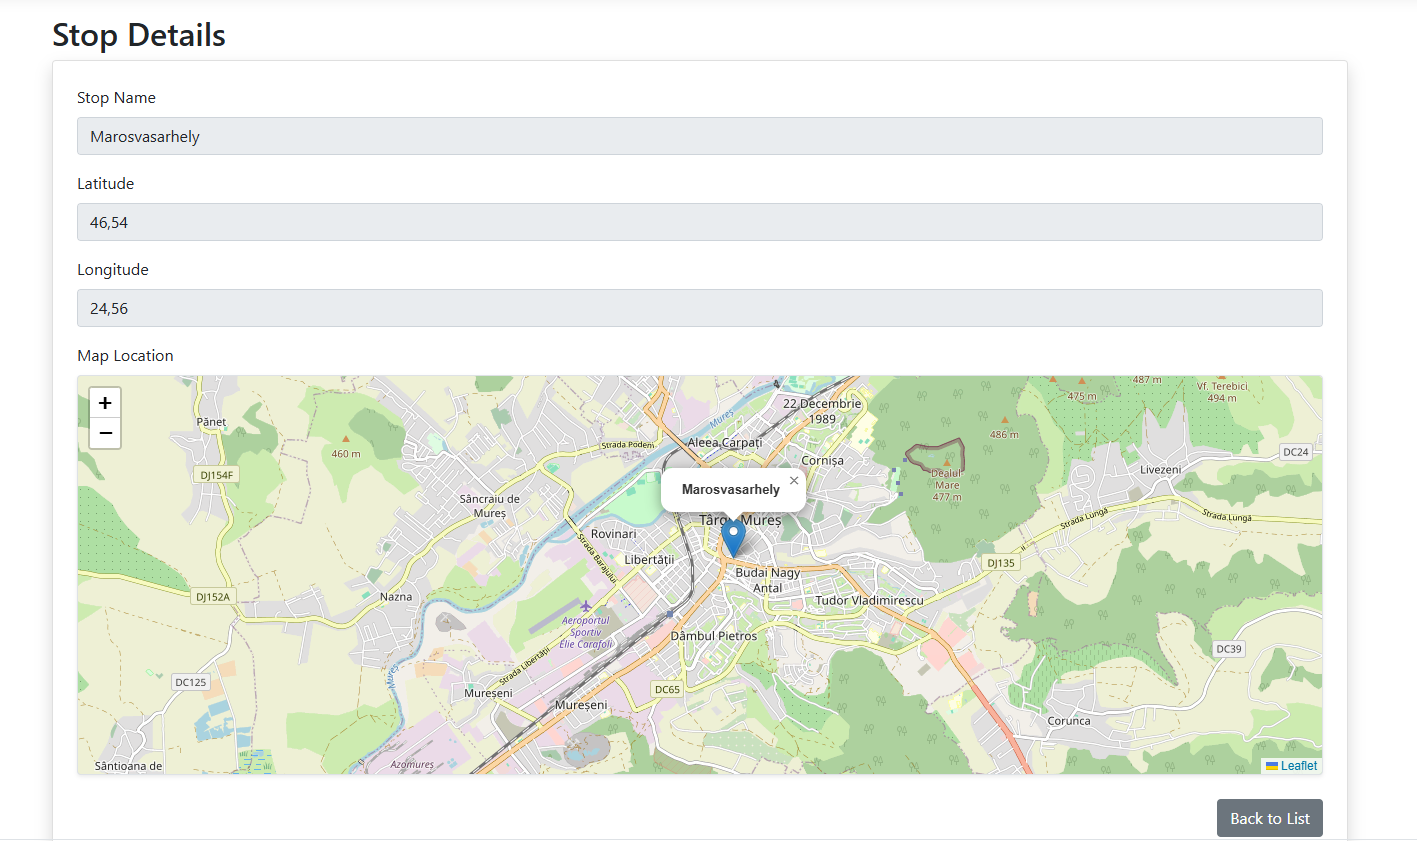
\includegraphics[width=1\textwidth]{Szakdolgozat/Mellekletek/StopDetail.PNG}
    \caption{Megálló részletes adatlapja felhasználói nézetben, térképes megjelenítéssel}
    \label{fig:stop-detail-user}
\end{figure}

A \ref{fig:stop-detail-user}. ábra egy megálló részletes adatlapját szemlélteti olyan formában, ahogyan azt egy általános felhasználó látja, aki a főmenüből navigált erre az oldalra.

Fontos megjegyezni, hogy adminisztrátori jogosultság esetén az ugyanilyen részletes nézet tartalmilag hasonló, azonban a térképes megjelenítés hiányzik belőle. Mivel az adminisztrátorok a megállók kezelését más, célzott nézetekből végzik (pl. a kezelőfelület táblázatos listájából kiindulva), a részletes oldal csupán kiegészítő információként szolgál számukra.


\subsubsection{Routes oldal}

A \texttt{Routes} felületen az elérhető útvonalak jelennek meg listázva, a felhasználók számára pedig megtekinthetők az útvonal részletei, beleértve a kiindulási és végállomást, valamint a köztes megállókat. Az adminisztrátorok ezen az oldalon hozzáadhatnak új útvonalakat, módosíthatják a meglévőket, vagy törölhetik azokat. Ezen felül lehetőség van megállók hozzárendelésére az adott útvonalhoz.

\subsubsection{Schedules oldal}

A \texttt{Schedules} oldalon a felhasználók a menetrendeket böngészhetik, amelyeket dátum, időpont, útvonal és a közlekedő busz szerint csoportosít a rendszer. Amennyiben az adott járaton van szabad ülőhely, lehetőség van jegyvásárlásra is. Az adminisztrátorok teljes körű menetrendkezelést végezhetnek: új menetrendeket adhatnak hozzá, szerkeszthetik vagy törölhetik a meglévőket, valamint hozzárendelhetik a kiválasztott útvonalakat és autóbuszokat.

\subsubsection{Ticket oldal}

A \texttt{Ticket} oldalon a felhasználók áttekinthetik az általuk megvásárolt jegyek listáját, és részletes információt kaphatnak az adott jegyhez tartozó menetrendről, az ülőhely számáról, valamint a QR kódos azonosítóról. Adminisztrátori nézetben az összes felhasználó által vásárolt jegyek megtekinthetők, továbbá lehetőség van keresésre és szűrésre is felhasználók szerint.

\subsubsection{Contact Us oldal}

A \texttt{Contact Us} oldal egy kapcsolatfelvételi űrlapot biztosít minden látogató számára, ahol név, e-mail cím és az üzenet szövege adható meg. Az elküldött üzenetek automatikusan elmentődnek az adatbázisba, és a rendszer egyidejűleg értesítést küld az adminisztrátornak e-mailben is.

\subsubsection{Adminisztrációs oldalak}

Az adminisztrátori jogosultsággal rendelkező felhasználók egy külön \texttt{Adminisztráció} legördülő menü segítségével érhetik el a rendszer admin funkcióit. A \texttt{Bus} menüpont alatt az autóbuszok adatai kezelhetők (például rendszám és kapacitás), míg az \texttt{Attachments} oldalon dokumentumok és egyéb fájlok feltöltésére és listázására van lehetőség. A \texttt{ToDoList} a rendszergazdák saját feladatait tartalmazza, míg az \texttt{Admin Messages} a felhasználóktól érkező üzenetek megtekintésére szolgál. A \texttt{Contact} menüpont alatt a felhasználói profilok érhetők el, és lehetőség van azok módosítására is. Végül a \texttt{Roles} oldalon a különböző szerepkörök – például egyszerű felhasználó vagy adminisztrátor – kezelése történik.



